% ==============================================================================
% CentraleSupélec Report Template
% ------------------------------------------------------------------------------
% Copyright-style notice and permissive use terms
%
% This template is intended for CentraleSupélec reports. It was made by
% Heitor Gama (heitor.gama@student-cs.fr) and adapted from an anonymous
% template that may have been made by past Brazilian students.
%
% This template is NOT official CentraleSupélec material. It is not endorsed,
% approved, maintained, or validated by the school, any department, or any
% course team. It cannot predict the formatting rules, submission constraints,
% AI-use policies, citation requirements, or grading preferences of a specific
% course, instructor, jury, or academic year.
%
% Use this template at your own risk. Heitor Gama is not responsible for any
% formatting issue, policy violation, missed requirement, grade penalty, or
% other consequence that may result from using, modifying, or distributing it.
%
% Permission is granted to use, copy, adapt, and distribute this template in
% any form, for any purpose, provided that this entire notice is kept at the
% top of the main .tex file in every copy or derivative version.
% ==============================================================================

% !TEX program = pdflatex
\pdfminorversion=6
\documentclass[a4paper,11pt]{report}

%====================== PACKAGES ======================

\usepackage[utf8]{inputenc}
\usepackage[T1]{fontenc}
% For French reports, uncomment this:
% \usepackage[french]{babel}
\usepackage{amsmath}
\usepackage{array}
\usepackage{booktabs}
\usepackage{float}
\usepackage{graphicx}
\usepackage{longtable}
\usepackage{siunitx}
\usepackage{tabularx}
\usepackage[most]{tcolorbox}
\usepackage{listings}
\usepackage{fancyhdr}
\usepackage{chngcntr}
\usepackage[numbers]{natbib}
\usepackage[
  top=3cm,
  bottom=2cm,
  left=1.5cm,
  right=1.5cm,
  headheight=3cm,
  headsep=0pt
]{geometry}
\usepackage{hyperref}

\graphicspath{{figures/}}

\hypersetup{
  colorlinks=true,
  linkcolor=blue,
  urlcolor=blue,
  citecolor=blue
}

\sisetup{
  detect-all,
  per-mode=symbol
}

% Keep report-class section numbers as 1, 2, 3... without chapter prefixes.
\counterwithout{section}{chapter}
\renewcommand{\thesection}{\arabic{section}}
\renewcommand{\thesubsection}{\thesection.\arabic{subsection}}
% Default LaTeX does not number subsubsections; this template does so only
% because it includes one explicit subsubsection example.
\setcounter{secnumdepth}{3}

%====================== TEMPLATE METADATA ======================

% Replace these fields for each new report.
\newcommand{\reporttitle}{Report Title: Concise Technical Subtitle}
\newcommand{\reportsubtitle}{Course, Project, Laboratory, or Conference Track}
\newcommand{\reportauthors}{First AUTHOR \\ Second AUTHOR \\ Third AUTHOR}
\newcommand{\reportaffiliation}{CentraleSupélec, Department or Research Group}
\newcommand{\reportsupervisors}{Advisor or Instructor Name(s)}
\newcommand{\reportdate}{\today}

% Logo file used in the centered header. Replace the PDF in figures/ or rename this path.
\newcommand{\institutionlogo}{%
  \IfFileExists{figures/institution-logo.pdf}{%
    
\includegraphics[height=2.6cm]{figures/institution-logo.pdf}%
  }{%
    \fbox{\parbox[c][2.2cm][c]{5.5cm}{\centering Institution logo}}%
  }%
}

%====================== PAGE STYLE ======================

\newcommand{\HRule}{\rule{\linewidth}{0.5mm}}

% On body pages, top=3cm, headheight=3cm, and headsep=0pt reserve one
% top band above the text; the logo is centered in that band.
\newcommand{\vcenterinhead}[1]{%
  \raisebox{0.5\dimexpr\headheight-\height\relax}{#1}%
}

\pagestyle{fancy}
\fancyhf{}
\newcommand{\titleheader}{\vcenterinhead{\institutionlogo}}
\newcommand{\bodyheader}{\vcenterinhead{\institutionlogo}}
\fancyhead[C]{\bodyheader}
\fancyfoot[C]{\thepage}
\renewcommand{\headrulewidth}{0pt}

%====================== REUSABLE ENVIRONMENTS ======================

\newcolumntype{Y}{>{\centering\arraybackslash}X}

\newtcblisting{pseudocodebox}{
  listing only,
  listing engine=listings,
  listing options={
    basicstyle=\ttfamily\small,
    numbers=left,
    breaklines=true,
    showstringspaces=false,
    keepspaces=true,
    columns=fullflexible
  },
  colback=gray!5,
  colframe=gray!50,
  boxrule=0.5pt,
  arc=2mm,
  left=1mm,
  right=1mm,
  top=1mm,
  bottom=1mm,
  breakable
}

\lstset{
  frame=single,
  basicstyle=\ttfamily\small,
  columns=fullflexible,
  breaklines=true
}

\newcommand{\aidisclosure}{%
  \phantomsection
  \addcontentsline{toc}{section}{Use of AI Tools}
  \noindent{\footnotesize\textbf{Use of AI Tools}}

  {\footnotesize
  \noindent This report may have used AI tools for limited support tasks such as drafting, editing, code review, formatting, literature organization, or checking consistency. The authors remain responsible for the accuracy of the technical content, the validity of the analysis, the interpretation of results, and the proper citation of all sources. Replace this paragraph with the disclosure required by your course, venue, or institution.
  }
}

%======================== DOCUMENT ========================

\begin{document}
\hypersetup{pageanchor=false}

\newgeometry{
  top=1.2cm,
  bottom=2cm,
  left=2cm,
  right=2cm,
  includehead,
  headheight=3cm,
  headsep=6mm
}

\begin{titlepage}
  \thispagestyle{fancy}
  \fancyhead[C]{\titleheader}
  \fancyfoot{}

  \begin{center}
    \vspace*{\fill}

    \HRule\\[0.4cm]
    {\huge\bfseries \reporttitle \\[0.4cm]}
    {\large\bfseries \reportsubtitle \\[0.4cm]}
    {\large \reportaffiliation \\[0.4cm]}
    {\large Supervisors: \reportsupervisors}
    \HRule\\[1.5cm]

    \vspace*{\fill}

    \begin{minipage}{0.45\textwidth}
      \begin{flushleft}\large
        \emph{Authors:}\\
        \reportauthors
      \end{flushleft}
    \end{minipage}

    \vfill

    {\large \reportdate}
  \end{center}
\end{titlepage}
\fancyhead[C]{\bodyheader}
\fancyfoot[C]{\thepage}

\restoregeometry

\clearpage
\pagenumbering{gobble}
\pagestyle{empty}
\newgeometry{top=2.2cm,bottom=2cm,left=2cm,right=2cm}

\noindent{\huge\bfseries Abstract\par}
\vspace{1em}
\noindent
This document is a non-official CentraleSupélec report template made by Heitor Gama for technical reports, lab write-ups, and project submissions. The source-code notice at the top of \texttt{main.tex} gives authorship, reuse, and liability details. The template provides a title page, abstract, table of contents, section structure, figures, tables, references, appendix examples, and an optional AI-use disclosure, but it is not school-approved and does not guarantee compliance with course-specific instructions. When adapting it, replace this paragraph with a concise abstract of roughly 150--250 words. You may adapt the abstract as a short paragraph right before the Introduction section for shorter reports.

\restoregeometry

\clearpage
\pagenumbering{gobble}
\pagestyle{empty}
\newgeometry{top=2.2cm,bottom=2cm,left=2cm,right=2cm}
\noindent{\huge\bfseries Contents\par}
\vspace{1em}
\makeatletter
\@starttoc{toc}
\makeatother
\restoregeometry

\newpage
\hypersetup{pageanchor=true}
\pagenumbering{arabic}
\pagestyle{fancy}
\setcounter{page}{1}

%====================== MAIN CONTENT ======================

\section*{Introduction}
\addcontentsline{toc}{section}{Introduction}

Use the introduction to move from the broad context to the precise contribution of the report. The first paragraph should identify the practical or scientific problem and explain why it is worth studying now. The second paragraph should define the scope of the work, including the system, data, experiment, corpus, or case study considered. The final paragraph should state the report's main objective and outline the organization of the remaining sections.

When adapting this template, replace generic claims with specific evidence and cite sources where readers would expect support. Use non-breaking spaces before cross-references and citations; the code examples below show the source command and the rendered result.

\begin{quote}\small
\verb|Figure~\ref{fig:sample_diagram}| renders as Figure~\ref{fig:sample_diagram}.\\
\verb|Table~\ref{tab:inputs}| renders as Table~\ref{tab:inputs}.\\
\verb|~\cite{Lamport1994}| renders as~\cite{Lamport1994}.
\end{quote}

Keep the introduction readable for a technically informed audience that may not share your exact specialization. If the work follows an assignment, laboratory, or project brief, describe the intellectual task rather than copying the prompt.

This sentence shows how to add a footnote with a project page, repository, or personal website\footnote{Available at \url{https://heitor-gama.com}.}.

\section{Background and Related Work}

Use this section for the background, definitions, standards, or previous work needed to read the report. The sample citations here demonstrate bibliography usage and should be replaced by sources that are actually relevant to the project \cite{Lamport1994,Mittelbach2004,Tufte2001}.

Keep citations close to the statement they support. For example, write that a method is standard~\cite{Mittelbach2004} in the relevant sentence rather than placing all references at the end of a section. Add bibliography entries to \texttt{references.bib}, and keep all entries in one consistent citation style and level of detail.

\section{Data, Materials, or Case Description}

Use this section to present inputs, materials, cases, or notation that need a compact reference. Table~\ref{tab:inputs} illustrates the expected pattern: introduce the table in the text, place \verb|\label{...}| immediately after \verb|\caption{...}|, include units, and discuss the table after it appears.

\begin{table}[H]
  \centering
  \caption{Template table for reporting inputs, parameters, or experimental conditions.}
  \label{tab:inputs}
  \begin{tabularx}{\textwidth}{lYYY}
    \toprule
    Item & Description & Value or Range & Note \\
    \midrule
    Input A & State what this variable represents. & \SI{10}{\meter} & Source or short note. \\
    Input B & Include units in the value or header. & \SIrange{1}{5}{\second} & Formatting note. \\
    Input C & Mark estimates clearly. & Estimated & Short explanatory note. \\
    \bottomrule
  \end{tabularx}
\end{table}

Tables should have captions that allow them to stand on their own. Put units in headers, align comparable numbers, and avoid excessive precision. Use \verb|booktabs| rules as in Table~\ref{tab:inputs}; avoid vertical rules unless they genuinely improve readability. If a table is too wide, reconsider whether all columns are necessary before reducing the font size.

\section{Methods}

Use the methods section for notation, equations, workflows, or procedures. Define notation before using it, keep variable names consistent, and cite a source when using a standard method.

\begin{equation}
  M = \frac{1}{n}\sum_{i=1}^{n} w_i x_i,
  \label{eq:weighted_metric}
\end{equation}
where \(M\) is the reported metric, \(x_i\) is an observation or component, \(w_i\) is a weight, and \(n\) is the number of observations. Replace Equation~\ref{eq:weighted_metric} with the central equation of the report and define every symbol immediately after the equation.

Displayed equations are part of the surrounding sentence and should carry the punctuation required by that sentence. In Equation~\ref{eq:weighted_metric}, the comma after the formula is intentional because the sentence continues with ``where''. If the sentence ends at the equation, place a period at the end of the displayed formula.

\subsection{Algorithm or Workflow}

Use a short algorithm description when implementation details affect the report. Prefer pseudocode that explains the logic rather than language-specific code. Use code in a particular programming language only when the point is to show that the implementation is simple or when syntax itself matters. Place longer code or configuration details in the appendix or a repository, and reference as in the main text, as in Appendix~\ref{app:supplementary}.

\begin{pseudocodebox}
inputs: values x_i and weights w_i
total_weight <- 0
weighted_sum <- 0

for each pair (x_i, w_i) in the inputs:
    total_weight <- total_weight + w_i
    weighted_sum <- weighted_sum + w_i * x_i

return weighted_sum / total_weight
\end{pseudocodebox}

\section{Results}

Use this section to place figures and tables close to the text that discusses them. Introduce each visual before it appears, then refer to it again when explaining what the reader should notice.

\begin{figure}[H]
  \centering
  % Prefer vector figures such as PDF for diagrams and plots.
  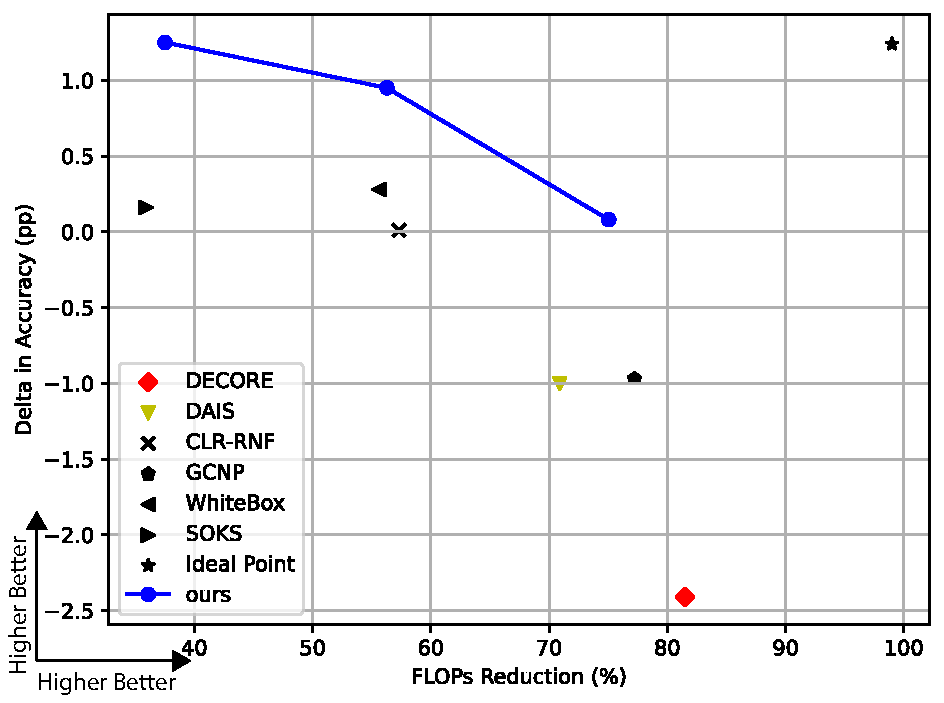
\includegraphics[width=0.45\textwidth]{figures/sample_figure.pdf}
  \caption{Example vector figure. The caption states what is shown and why the visual encoding remains readable without relying only on color.}
  \label{fig:sample_diagram}
\end{figure}

Every figure and every table should be referenced in the text, as done here with Figure~\ref{fig:sample_diagram} and Table~\ref{tab:inputs}. Prefer vector outputs such as PDF for plots, diagrams, and schematics; reserve raster formats such as PNG or JPEG for photographs or image data. Keep all figure text in the same language as the report; if a source figure is in another language, reconstruct or redraw it from the original source when necessary. Always label plot axes and include units directly in the axis labels, for example \(t\) (s) or power (MW). A hard title inside a plot can usually be omitted because the caption identifies the figure; add one only when it helps, such as when several subplots need short internal titles. Use color carefully: a colorblind reader should still understand the plot, so combine color with line style, markers, labels, direct annotations, or texture. Do not use red/green contrast as the only signal.

\section{Discussion}

Use the discussion section when it improves the structure of the report. Keep paragraphs short enough to scan, refer back to figures, tables, and equations instead of repeating them, and separate this section from the conclusion if both are included.

\section{Limitations and Future Work}

Use this section when limitations or next steps would otherwise make the conclusion too long. Keep limitations specific and traceable to the report, and format future work as a short set of concrete directions rather than an open-ended wish list.

\section*{Conclusion}
\addcontentsline{toc}{section}{Conclusion}

Use the conclusion for the final short section of the report. Avoid introducing new figures, tables, acronyms, or unexplained references here unless the course instructions require them.

\section*{Acknowledgements}
\addcontentsline{toc}{section}{Acknowledgements}

Use this optional section to thank supervisors, instructors, collaborators, technical staff, funding sources, or people who provided feedback but are not listed as authors. Keep acknowledgements concise and check whether the course or venue expects them to be included, omitted, or anonymized.

\vfill
% Comment out the following line if you do not want the AI disclosure note.
\aidisclosure

%====================== REFERENCES ======================

\clearpage
\phantomsection
\addcontentsline{toc}{section}{References}
\renewcommand{\bibsection}{\noindent{\huge\bfseries References\par}\vspace{1em}}
\bibliographystyle{plainnat}
\bibliography{references}

%====================== APPENDIX ======================

\clearpage
\appendix
\setcounter{section}{0}
\renewcommand{\thesection}{\Alph{section}}
\renewcommand{\thesubsection}{\thesection.\arabic{subsection}}
\phantomsection
\addcontentsline{toc}{section}{Appendix}
\noindent{\huge\bfseries Appendix\par}
\vspace{1em}

\section{Supplementary Material}\label{app:supplementary}

Use appendices for material that supports reproducibility or auditability but would interrupt the main argument. Examples include long derivations, extended tables, additional figures, survey instruments, data dictionaries, parameter files, or implementation notes.

\begin{longtable}{p{0.25\textwidth}p{0.65\textwidth}}
  \caption{Template data dictionary or symbol table.}
  \label{tab:data_dictionary}\\
  \toprule
  Field or Symbol & Meaning \\
  \midrule
  \endfirsthead
  \toprule
  Field or Symbol & Meaning \\
  \midrule
  \endhead
  \(x_i\) & Observation, sample, design variable, or measured quantity. \\
  \(w_i\) & Weight, coefficient, or confidence factor associated with \(x_i\). \\
  \(M\) & Aggregate metric reported in the main text. \\
  \bottomrule
\end{longtable}

\section{Reproducibility Checklist}

Before submitting, replace this checklist with course-specific requirements or remove it. Common formatting checks include: every figure and table is referenced, captions are readable, units are explicit, sources are cited, and the AI disclosure is adjusted to the rules of the course.

\subsection{Checklist Notes}

Use subsections in the appendix when they group several related details under a clear topic. This heading is numbered as B.1 because it is the first subsection of Appendix~B.

\subsubsection{Appendix Heading Granularity}

Appendix subsubsections are useful for long derivations, implementation details, or repeated experiment variants. Do not split the appendix into many tiny headings just to make it look comprehensive; readers use the appendix to audit details, so its organization should remain compact and searchable.

\end{document}
